\chapter{Colour}\label{ch:colour}

\section{Match the colour map to the data}
\begin{tabularx}{\linewidth}{@{}lXl@{}}
\toprule
Data & Colour map & Name in \texttt{carto} \\
\midrule
Ordered values, such as snow days & Sequential: one steady change in lightness & \texttt{SEQUENTIAL} (batlow) \\
Values around a meaningful zero, such as anomalies & Diverging: two hues meeting at a neutral colour & \texttt{DIVERGING} (vik) \\
Categories, such as land cover & Qualitative: distinct colours & \texttt{QUALITATIVE} (Okabe-Ito) \\
\bottomrule
\end{tabularx}

\begin{figure}[H]\centering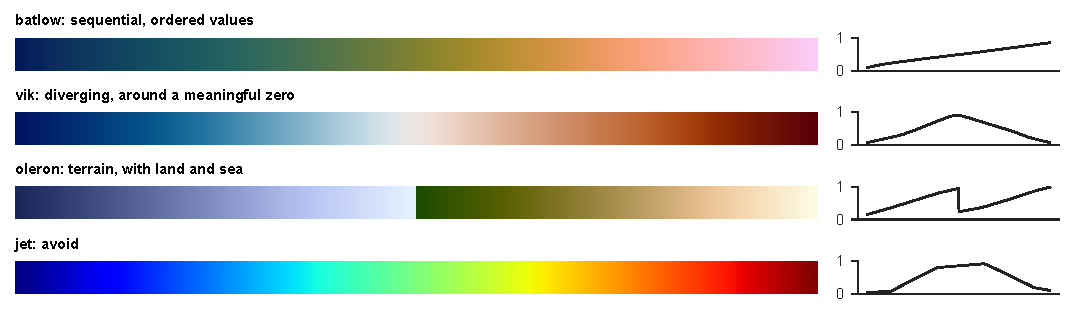
\includegraphics[width=\linewidth]{fig_colours.pdf}
\caption{Colour maps (left) with their lightness (right). Batlow rises fairly steadily. Jet rises and falls, creating false edges in smooth data, and fails for many colour-blind readers.}\end{figure}

\begin{figure}[H]\centering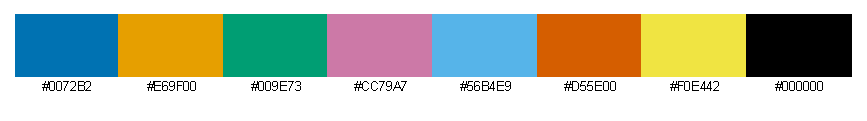
\includegraphics[width=\linewidth]{fig_palette.pdf}
\caption{The qualitative palette, chosen to stay distinct for common colour-vision deficiencies.}\end{figure}

\section{Rules}
\begin{enumerate}
\item Centre a diverging map on the meaningful value, with \texttt{vmin=-lim, vmax=lim}.
\item Fix limits across panels you want compared. Otherwise, the same colour means different values.
\item Stretch by percentiles for display, and say so, because a few bright pixels would otherwise wash out the rest:
\begin{lstlisting}[language=Python]
lo, hi = np.nanpercentile(a, [2, 98])
\end{lstlisting}
\item Never let colour alone carry meaning: add labels or hatching where you can.
\item Print or view in greyscale once, to test the map.
\end{enumerate}

\section{Over imagery}
Satellite images are busy, so plain labels get lost. \texttt{outlined()} adds a dark edge to text, and \texttt{mark()} draws numbered white circles, which read on any background. Explain the numbers in the caption or a table. This also suits print, since long place names no longer cover the data.
\snippetcaption{research\_helpers/carto.py, mark(), lines 102--107}
\begin{lstlisting}[firstnumber=102]
def mark(ax, points, transform=None, size=7):
    """Numbered markers with a halo, readable over any image. points is a list of (number, x, y); a caption or key explains them."""
    transform = transform or ccrs.PlateCarree()
    for n, x, y in points:
        ax.text(x, y, str(n), transform=transform, ha="center", va="center", fontsize=size, fontweight="bold", color="black", zorder=20,
                bbox=dict(boxstyle="circle,pad=0.25", facecolor="white", edgecolor="black", linewidth=0.5))
\end{lstlisting}

\snippetcaption{research\_helpers/carto.py, outlined(), lines 110--112}
\begin{lstlisting}[firstnumber=110]
def outlined(ax, x, y, text, transform=None, size=7, color="white"):
    """A place label with an outline, for use over imagery."""
    return ax.text(x, y, text, transform=transform or ccrs.PlateCarree(), fontsize=size, color=color, zorder=19, path_effects=[pe.withStroke(linewidth=1.8, foreground="black")])
\end{lstlisting}

